\addcontentsline{toc}{chapter}{Занятие 2. Характеристики случайного процесса}
\chapter*{Занятие 2. Характеристики случайного процесса}

\addcontentsline{toc}{section}{Контрольные вопросы и задания}
\section*{Контрольные вопросы и задания}

\subsubsection*{Приведите определение случайного процесса.}

Случайный процесс $ \xi \left( t \right), \, t \in T$ ---
это параметризированная совокупность случайных величин.

\subsubsection*{Что называют конечномерными распределениями случайного процесса?}

$ \left\{ \mu_{t_1, \dotsc, t_n}; \, t_1, \dotsc, t_n \in T, \, n \geq 1 \right\} $ ---
набор конечномерных распределений процесса $ \xi $, где $ \mu_{t_1, \dotsc, t_n}$ ---
распределение вектора $ \left( \xi \left( t_1 \right), \dotsc, \xi \left( t_n \right) \right) $ в
$ \mathbb{R}^n$,
то есть для борелевского
$ \Delta \in \mathcal{B} \left( \mathbb{R}^n \right), \,
  \mu_{t_1, \dotsc, t_n} \left( \Delta \right) =
  P \left\{
    \left( \xi \left( t_1 \right), \dotsc, \xi \left( t_n \right) \right) \in \Delta
  \right\} $.

\subsubsection*{Приведите определение функции математического ожидания,
                дисперсии и ковариационной функции случайного процесса.}

$m \left( t \right) = M \xi \left( t \right), \, t \in T$ --- функция среднего.

$D \xi \left( t \right), \, t \in T$ --- функция дисперсии.

$K \left( t, s \right) =
  M \left[ \xi \left( t \right) - m \left( t \right) \right] \cdot
  \left[ \xi \left( s \right) - m \left( s \right) \right], \, t, s \in T$ ---
функция ковариации.

\addcontentsline{toc}{section}{Аудиторные задачи}
\section*{Аудиторные задачи}

\subsubsection*{2.2}

\textit{Задание.}
Пусть
$$ \xi \left( t \right) =
  X \cdot e^{-t}, \,
  t > 0,$$
где $X$ --- случайная величина,
которая имеет нормальное распределение с параметрами $a, \, \sigma^2$.
Найдите математическое ожидание, дисперсию,
ковариационную функцию и одномерную плотность распределения случайного процесса
$ \xi =
  \left\{ \xi \left( t \right), \, t > 0 \right\} $.

\textit{Решение.}
Сейчас $T = \left( 0, \infty \right) $.

Случайная величина $X$ имеет распределение $N \left( a, \sigma^2 \right) $.
Нужно найти $M \xi \left( t \right) = m \left( t \right), \, D \xi \left( t \right) $,
ковариационную функцию $K \left( t, s \right) $ и одномерную плотность распределения
$p_{ \xi } \left( t \right) $.

Найчнём с математического ожидания
$$m \left( t \right) =
  M \left( X \cdot e^{-t} \right) =
  e^{-t} MX =
  e^{-t} \cdot a.$$

Далее ---
функция дисперсии $D \xi \left( t \right) = D \left( X \cdot e^{-t} \right) = e^{-2t} \cdot DX$.
Дисперсия $X$ --- известная: $e^{-2t} \cdot DX = e^{-2t} \cdot \sigma^2$.

Далее ---
ковариационная функция
$$K \left( t, s \right) =
  M \left[ \xi \left( t \right) - m \left( t \right) \right] \cdot
  \left[ \xi \left( s \right) - m \left( s \right) \right] =
  cov \left[ \xi \left( t \right), \xi \left( s \right) \right].$$
Вместо $ \xi \left( t \right), \, \xi \left( s \right) $ подставляем их значения
$$cov \left[ \xi \left( t \right), \xi \left( s \right) \right] =
  cov \left( Xe^{-t}, Xe^{-s} \right).$$
Множители выносятся
$$cov \left( Xe^{-t}, Xe^{-s} \right) =
  e^{-t - s} cov \left( X, X \right) =
  e^{-t - s} DX =
  e^{-t - s} \sigma^2.$$

Последнее ---
это плотность $ \xi \left( t \right) \sim N \left( e^{-t} a, \, e^{-2t} \sigma^2 \right) $.

Нужно написать нормальную плотность с заданными математическим ожиданием и дисперсией
$$p_{ \xi \left( t \right) } \left( x \right) =
  \frac{1}{ \sqrt{2 \pi e^{-2t} \sigma^2}} \cdot
  e^{- \frac{ \left( x - e^{-t} a \right)^2}{2e^{-2t} \sigma^2}}.$$

Траектория процесса изображена на рисунке \ref{fig:22}
и имеет разный вид в зависимости от значения случайной величины $X$.

\begin{figure}[h!]
  \centering
  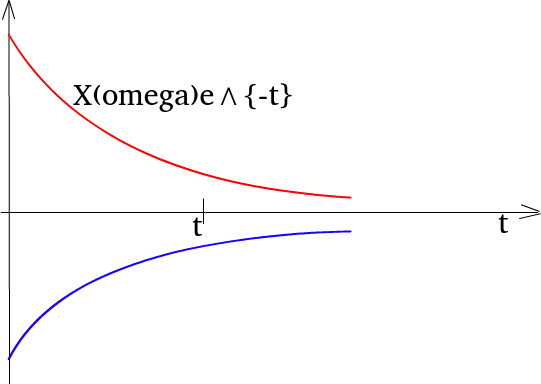
\includegraphics[width=.4\textwidth]{./pictures/2_2.png}
  \caption{Траектория процесса}
  \label{fig:22}
\end{figure}

\addcontentsline{toc}{section}{Домашнее задание}
\section*{Домашнее задание}
